\chapter{Encoder BCD}

\section{Encoder BCD}
\paragraph{Traccia}
Progettare, implementare in VHDL e testare mediante simulazione una rete che, data in ingresso una stringa binaria X di 10 bit X9 X8 X7 X6 X5 X4 X3 X2 X1 X0 che corrisponde alla rappresentazione decodificata di una cifra decimale (cioè, una rappresentazione in cui ogni stringa contiene un solo bit alto), fornisce in uscita la rappresentazione Y della cifra mediante codifica Binary-Coded Decimali (BCD). 

\subsection{Architettura}
L'\textit{encoder} è una macchina combinatoria che realizza una funzione di corrispondenza ben definita tra ingresso e uscita. In Figura \ref{fig:encoder_arch} è mostrata l'architettura della soluzione.

\begin{figure}[H]
    \centering
    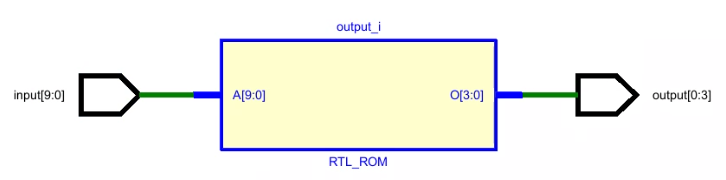
\includegraphics[width=15cm]{immagini/esercizio2/schema_2.1.png}
    \caption{Architettura encoder}
    \label{fig:encoder_arch}
\end{figure}

L'implementazione è stata realizzata mediante un processo con il costrutto \textit{case-when} ed è riportata nel listato \ref{encoder}.

\begin{lstlisting}[language=VHDL, label=encoder, caption=Encoder BCD]
library IEEE;
use IEEE.STD_LOGIC_1164.ALL;
entity encoder is port ( 
    input: in STD_LOGIC_VECTOR (9 downto 0);
    output: out STD_LOGIC_VECTOR (0 to 3)
  );
end encoder;

architecture Behavioral of encoder is

begin
    process(input)
        begin 
        case input is 
            when "0000000001" => output <="0000";
            when "0000000010" => output <="0001";
            when "0000000100" => output <="0010";
            when "0000001000" => output <="0011";
            when "0000010000" => output <="0100";
            when "0000100000" => output <="0101";
            when "0001000000" => output <="0110";
            when "0010000000" => output <="0111";
            when "0100000000" => output <="1000";
            when "1000000000" => output <="1001";
            when others =>output<="----";
            end case;   
    end process;    
end Behavioral;
\end{lstlisting}

\subsection{Testing}
Essendo il numero di input limitato, è stato possibile effettuare un testing esaustivo: ogni input è una stringa che contiene un solo bit alto. Per ogni test sono stati verificati gli output attesi, mentre l'output della simulazione è presente in Figura \ref{fig:Simulazione encoder}
Il \textit{testbench} è presente nel listato \ref{tb_encoder}.
\begin{lstlisting}[language=VHDL, label=tb_encoder, caption=Simulazione encoder]
library IEEE;
use IEEE.STD_LOGIC_1164.ALL;

entity encoder_TB is
end encoder_TB;
architecture Behavioral of encoder_TB is

component encoder is 
    Port(
        input: in STD_LOGIC_VECTOR (9 downto 0);
        output: out STD_LOGIC_VECTOR (0 to 3)
    );
end component;

signal s_input: STD_LOGIC_VECTOR(9 downto 0);
signal s_output: STD_LOGIC_VECTOR(0 to 3);

begin
  uut: encoder
    Port map ( 
      input=>s_input,
      output=>s_output
    );

test_bench: process
begin
    wait for 100 ns;

    s_input<="0000000001";
    wait for 10 ns;
    assert s_output = "0000"
    report "errore";
    wait for 10 ns;

    s_input<="0000000010";
    wait for 10 ns;
    assert  s_output = "0001"
    report "errore 1";
    wait for 10 ns;

    s_input<="0000000100";
    wait for 10 ns;
    assert  s_output = "0010"
    report "errore";
    wait for 10 ns;

    s_input<="0000001000";
    wait for 10 ns;
    assert  s_output = "0011"
    report "errore";
    wait for 10 ns;

    s_input<="0000010000";
    wait for 10 ns;
    assert  s_output = "0100"
    report "errore";
    wait for 10 ns;

    s_input<="0000100000";
    wait for 10 ns;
    assert  s_output = "0101"
    report "errore";
    wait for 10 ns;
    
    s_input<="0001000000";
    wait for 10 ns;
    assert  s_output = "0110"
    report "errore";
    wait for 10 ns;

    s_input<="0010000000";
    wait for 10 ns;
    assert  s_output = "0111"
    report "errore";
    wait for 10 ns;
    
    s_input<="0100000000";
    wait for 10 ns;
    assert  s_output = "1000"
    report "errore";
    wait for 10 ns;

    s_input<="1000000000";
    wait for 10 ns;
    assert  s_output = "1001"
    report "errore";
    wait;
end process;
end Behavioral;
\end{lstlisting}

\begin{figure}[H]
    \centering
    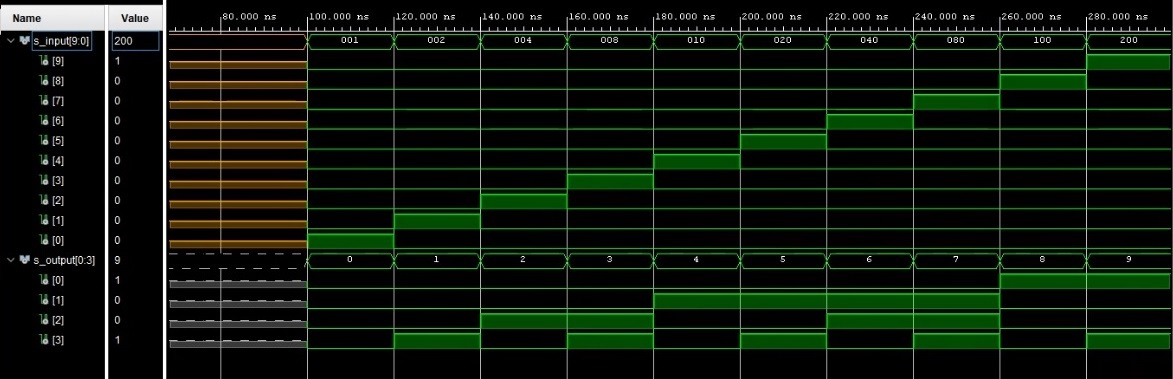
\includegraphics[width=16cm]{immagini/esercizio2/output_simulazione_2.1.jpg}
    \caption{Output della simulazione}
    \label{fig:Simulazione encoder}
\end{figure}

\section{Sintesi su scheda}
\paragraph{Traccia} 
Sintetizzare ed implementare su board il progetto dell’encoder BCD utilizzando gli switch per fornire la stringa X in ingresso, e i led per visualizzare Y. Nel caso in cui si utilizzi una board dotata di soli 8 switch, è possibile sviluppare il progetto considerando X di soli 8 bit (la macchina sarà allora in grado di fornire in uscita la rappresentazione BCD delle cifre decimali da 0 a 7).

\subsection{Implementazione}
In questo caso, la macchina resta completamente combinatoria e, pertanto, sono stati mappati gli switch della scheda direttamente sugli input dell'encoder. Una dimostrazione visiva del risultato è riportata nel file \textit{2.2.mkv} nella sezione materiale multimediale.

\section{Sintesi su scheda}
\paragraph{Traccia}
Utilizzare un display a 7 segmenti per visualizzare la cifra decimale codificata da Y (pilotare opportunamente i catodi del display).

\subsection{Implementazione}
Per la sintesi è stata creata un'unità dedicata \textit{Encoder\_OnBoard} (la cui implementazione è presente nel listato \ref{encoder_on_board}), tale unità utilizza il componente \textit{Encoder} sviluppato in precedenza, e si occupa di interagire con i segnali della scheda. In particolare, viene eseguita l'assegnazione degli input sugli switch della scheda e degli output sul display. Per il display è stato utilizzato il componente \textit{cathod\_manager} la cui interfaccia è riportata nel listato \ref{cathod_manager}.

\begin{lstlisting}[language=VHDL, label=cathod_manager, caption=Interfaccia cathod manager]
entity cathodes_manager is
    Port (
        value : in  STD_LOGIC_VECTOR (3 downto 0); --dato da mostrare sulla cifra del display
        dot : in  STD_LOGIC; --punto
        cathodes_dot : out  STD_LOGIC_VECTOR (7 downto 0)); --indica i 7 catodi + il punto
end cathodes_manager;
\end{lstlisting}

\begin{lstlisting}[language=VHDL, label=encoder_on_board, caption=Implementazione Encoder\_OnBoard]
library IEEE;
use IEEE.STD_LOGIC_1164.ALL;

entity Encoder_onBoard is
    Port (
        input : in STD_LOGIC_VECTOR(9 downto 0);
        led : out STD_LOGIC_VECTOR(3 downto 0);
        catodi : out STD_LOGIC_VECTOR(7 downto 0);
        anodi : out STD_LOGIC_VECTOR(7 downto 0)
    );
end Encoder_onBoard;

architecture Behavioral of Encoder_onBoard is

   component encoder
       Port (
         input: in STD_LOGIC_VECTOR (9 downto 0);
         output: out STD_LOGIC_VECTOR (3 downto 0)
       );
   end component;


   component cathodes_manager
       Port(
          value : in std_logic_vector(3 downto 0);
          dot : in std_logic;
          cathodes_dot : out std_logic_vector(7 downto 0)
       );
   end component;

    signal ytemp : std_logic_vector (3 downto 0);
    signal dot : std_logic;
    
begin

    dot <= '1';  --decido di voler illuminare il punto accanto alla cifra
    anodi <=(others=>'0'); --decido di voler illuminare tutte le cifre dei due display (anodi 0-attivi)
    led <= ytemp;

    enc: Encoder port map(
            input => input,
            output => ytemp
        );

    cat: cathodes_manager port map(
            value => ytemp,
            dot => dot,
            cathodes_dot => catodi
        );

end Behavioral;
\end{lstlisting}